\chapter{Realizzazione file system}
\section{Struttura del File System}
\subsection{Architettura Generale del File System}
\dfn{File System}{La struttura di un file system è organizzata in livelli che interagiscono per fornire un'interfaccia tra l'utente e i dispositivi di memoria di massa. Ecco i principali componenti:}

\begin{itemize}
    \item \textbf{Utente}: Accede ai file tramite comandi (es. \texttt{ls}, \texttt{dir}, \texttt{mv}) o programmi applicativi.
    \item \textbf{File System Logico}: Fornisce i nomi simbolici per i file e struttura le directory.
    \item \textbf{Modulo Organizzazione dei File}: Gestisce i file a livello di blocchi e fornisce l'interfaccia nomi/blocchi.
    \item \textbf{Controllo I/O}: Coordina le operazioni di input/output interfacciandosi con i driver dei dispositivi.
    \item \textbf{Dispositivi di Memoria}: Hard disk e controller del disco gestiscono fisicamente la lettura/scrittura dei blocchi.
\end{itemize}

\nt{
    Ogni livello semplifica le operazioni per quello superiore, isolando i dettagli tecnici della gestione dei dispositivi.
}

\subsection{Interazione tra Utente e Sistema Operativo}
L'utente interagisce con il file system tramite comandi o interfacce grafiche. Il SO, attraverso i moduli interni, traduce i nomi simbolici dei file in operazioni sui blocchi fisici del disco.

\section{Metodi di Allocazione dei File}
\subsection{Introduzione}
Il file system utilizza l'hard disk come dispositivo di memoria di massa. Il disco è visto dal sistema operativo come un grande array di blocchi, dove ogni blocco può contenere, ad esempio, 1024 byte (ma altri valori tra 256 e 4096 byte sono possibili).

\nt{
    Le operazioni di lettura e scrittura avvengono sempre su blocchi interi, identificati tramite il loro numero.
}

\subsection{Gestione dei Blocchi}
Quando un file supera la dimensione di un singolo blocco, il SO lo divide su più blocchi, tenendo traccia di quali blocchi appartengono al file. Per ogni file, il sistema mantiene una struttura interna che ne memorizza tutti gli attributi, come posizione, dimensione, e permessi.

\nt{
    Esistono tre principali metodi per allocare i blocchi ai file:
    \begin{itemize}
        \item Allocazione Contigua
        \item Allocazione Concatenata
        \item Allocazione Indicizzata
    \end{itemize}
}


\subsection{Allocazione Contigua}
Con l'allocazione contigua, ogni file è memorizzato in blocchi contigui sull'hard disk. Questo metodo richiede:
\begin{itemize}
    \item Il numero del primo blocco del file.
    \item La quantità di blocchi contigui occupati dal file (opzionale, poiché la dimensione del file è già memorizzata tra i suoi attributi).
\end{itemize}

\nt{
    Questo metodo era comunemente utilizzato nei sistemi IBM VM/CMS.
}

\subsubsection{Vantaggi}
\begin{itemize}
    \item Accesso rapido: Poiché i blocchi sono contigui, il tempo di ricerca è minimo.
    \item Semplicità: La gestione dei file risulta semplice, dato che i blocchi sono consecutivi.
\end{itemize}

\subsubsection{Svantaggi}
L'allocazione contigua presenta numerosi svantaggi, simili a quelli dell'allocazione contigua della memoria primaria. Per esempio:
\begin{itemize}
    \item È necessario trovare uno spazio libero sul disco costituito da una serie di blocchi adiacenti.
    \item Occorre adottare una strategia per scegliere il buco libero in cui memorizzare un file (ad esempio: \textit{first fit}, \textit{best fit}, \textit{worst fit}).
    \item Il disco è soggetto a frammentazione esterna.
    \item A lungo andare, sarà necessaria una ricompattazione periodica del disco, un'operazione molto più costosa rispetto alla ricompattazione della memoria primaria.
\end{itemize}

\nt{
Se anche troviamo spazio sufficiente per allocare un file, il problema si presenta nel caso in cui la dimensione del file aumenti. In questo caso:
\begin{itemize}
    \item Siamo costretti a riallocarlo, un'operazione costosa in termini di lettura e riscrittura dei blocchi.
    \item Oppure possiamo sovradimensionare il file, ad esempio allocandogli 10 blocchi anche se ne occupa solo 5. Tuttavia, questa scelta aggrava il problema della frammentazione interna (già presente a causa dell'ultimo blocco parzialmente occupato).
\end{itemize}
}
\begin{figure}[h] \centering 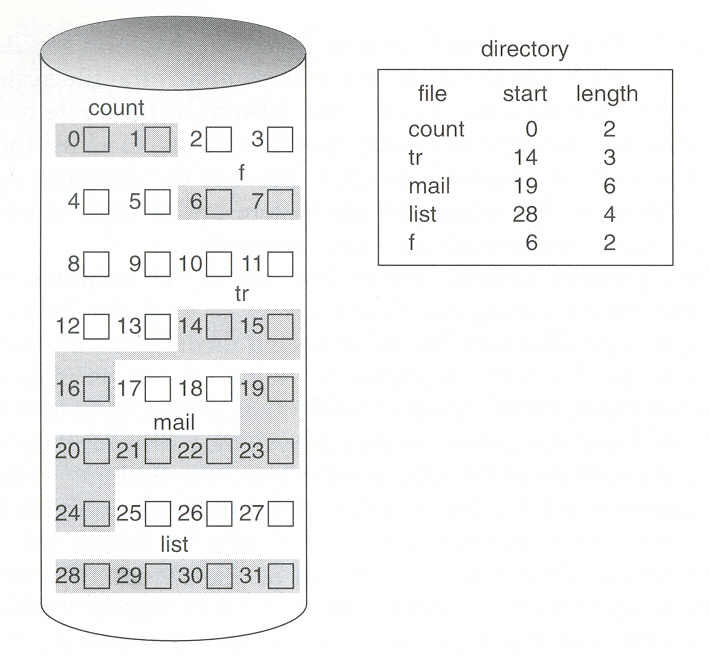
\includegraphics[width=0.33\linewidth]{images/allocazione_contigua_Scheme.png} \caption{Allocazione contigua} \label{fig:14.4} \end{figure}


\clm{Osservazioni sull'allocazione contigua}{}{
In definitiva, l'allocazione contigua presenta problemi analoghi a quelli visti per la memoria primaria:
\begin{itemize}
    \item Frammentazione esterna.
    \item Riallocazioni costose in caso di crescita dei file.
    \item Problemi di sovradimensionamento.
\end{itemize}
}

\subsection{Allocazione concatenata}

Per superare i limiti dell'allocazione contigua, si adotta un approccio simile a quello usato per la memoria primaria: l'allocazione concatenata.

\begin{itemize}
    \item In questo metodo, i dati del file sono distribuiti in una catena di blocchi non contigui.
    \item Ogni blocco contiene, negli ultimi byte, un puntatore al blocco successivo (numero del blocco).
    \item Per individuare i blocchi di un file, è sufficiente memorizzare, tra gli attributi del file, il numero del blocco iniziale.
\end{itemize}

\nt{
Opzionalmente, possono essere memorizzati anche:
\begin{itemize}
    \item Il numero totale di blocchi usati.
    \item Il numero del blocco finale.
\end{itemize}
}

\begin{figure}[h] \centering 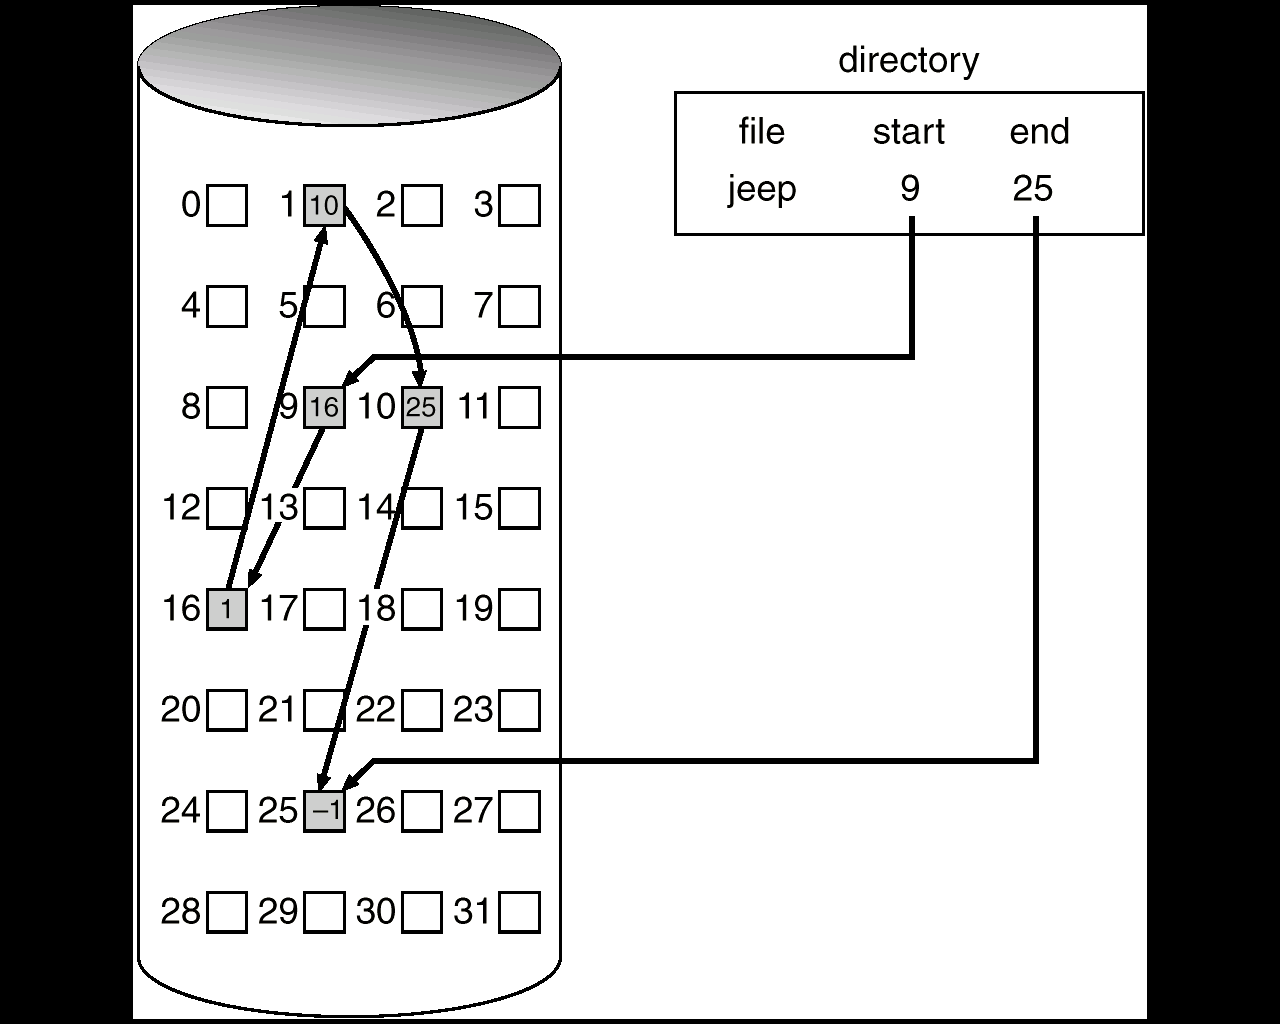
\includegraphics[width=0.50\linewidth]{images/allocazione_concatenata.png} \caption{Allocazione concatenata} \end{figure}

\nt{
Nell’ultimo blocco della catena, lo spazio destinato al puntatore al blocco successivo viene riempito con un numero negativo o con il valore \texttt{0}, per indicare che si tratta dell’ultimo blocco del file.
}

\subsection{Vantaggi dell’Allocazione Concatenata}
\begin{itemize}
    \item Non richiede blocchi contigui, eliminando la necessità di ricompattare il disco.
    \item Non si verifica frammentazione esterna.
    \item Qualsiasi blocco libero può essere utilizzato per memorizzare una porzione del file.
\end{itemize}

\subsection{Problemi dell’Allocazione Concatenata}
\begin{itemize}
    \item Una piccola porzione di ogni blocco viene occupata dal puntatore al blocco successivo (ad esempio, 4 byte in un blocco da 512 byte, causando uno spreco dello 0,78\%).
    \item L’accesso diretto al file può risultare altamente inefficiente:
          \begin{itemize}
              \item Per accedere all’n-esimo blocco, possono essere necessari n accessi al disco.
              \item Ogni blocco deve essere letto sequenzialmente per individuare il successivo.
          \end{itemize}
    \item Il sistema è poco affidabile: 
          \begin{itemize}
              \item Se un blocco del file viene danneggiato, si perde tutta la parte di file a partire dal blocco danneggiato.
          \end{itemize}
\end{itemize}

\subsection{Possibili Soluzioni ai Problemi}
\begin{itemize}
    \item Utilizzare \textbf{liste doppiamente concatenate}, memorizzando anche un puntatore al blocco precedente. Questo consente di recuperare i dati successivi in caso di danneggiamento di un blocco, risalendo la catena all’indietro.
    \item Memorizzare in ogni blocco il nome del file e la posizione del blocco nella catena. In questo modo, scandendo tutti i blocchi del disco, è possibile recuperare i blocchi persi (a costo di un aumento dello spazio occupato in ogni blocco).
    \item Non usare blocchi singoli, \textbf{ma considerare tutto l’HD formato da cluster di blocchi }
    \item Ad esempio, ciascun cluster puo’ essere composto da 4 blocchi del disco adiacenti, e avere quindi una dimensione 4 Kbyte (se i singoli blocchi sono da 1024 byte).
    \item in pratica è come lavorare con blocchi di dimensione più grossa, per cui:
    \begin{itemize}
        \item i puntatori ai blocchi successivi occupano una percentuale minore dello spazio
        \item i tempi di accesso al file diminuiscono, perchè dobbiamo riposizionare meno volte la testina di lettura
        \item meno spazio viene sprecato per i puntatori, però:
        \item aumenta la frammentazione interna
    \end{itemize}
\end{itemize}

\subsection{Allocazione concatenata: la variante della FAT}

\subsubsection{Introduzione alla FAT}
\nt{
Sebbene l’allocazione concatenata presenti gravi difetti, una sua variante molto efficiente, la \textbf{File Allocation Table} (FAT), è stata ampiamente adottata nei sistemi MS-DOS, OS/2 ed è ancora disponibile nei sistemi Windows come alternativa a NTFS.
}

La FAT è un’area situata all’inizio del disco (in pratica un array) in cui:
\begin{itemize}
    \item L’indice di ogni \textit{entry} corrisponde a un blocco del disco.
    \item Ogni entry contiene il numero del blocco successivo nella catena.
    \item Le entry contenenti il valore \texttt{0} rappresentano blocchi liberi.
\end{itemize}

\subsubsection{Funzionamento della FAT}
\begin{itemize}
    \item La FAT registra lo stato di allocazione di tutti i blocchi dell’hard disk e riproduce la lista concatenata dei blocchi di ciascun file.
    \item Se il blocco $I$ di un file punta al blocco $N$, allora la $I$-esima entry della FAT contiene il numero $N$.
    \item Se l’ultimo blocco di un file è il numero $J$, la $J$-esima entry della FAT contiene un \textit{marker} speciale che indica la fine del file.
\end{itemize}

\ex{Esempio di FAT}{
Per un file denominato \texttt{test}, basta memorizzare tra i suoi attributi il numero del primo blocco (ad esempio, 217). Per individuare gli altri blocchi che contengono i dati del file \texttt{test}, si utilizza il numero del primo blocco come indice nella FAT e si segue la catena di puntatori all’interno della FAT.
}

\subsubsection{Vantaggi della FAT}
\begin{itemize}
    \item Per garantire un accesso efficiente, la FAT viene mantenuta costantemente in RAM.
    \item Questo migliora sensibilmente l’accesso diretto ai file: per risalire all’$n$-esimo blocco di un file, basta seguire la catena di puntatori nella FAT (ossia leggere celle in RAM) invece di accedere ai blocchi fisici sul disco.
    \item Il sistema è più sicuro: se un blocco viene perso, la catena di blocchi è comunque riprodotta nella FAT.
    \item La gestione dei blocchi liberi è automatica: ogni entry contenente \texttt{0} rappresenta un blocco libero.
\end{itemize}

\subsubsection{Svantaggi della FAT}
\begin{itemize}
    \item La FAT occupa spazio in memoria principale (MP):
          \begin{itemize}
              \item Si tratta di un array con un numero di entry uguale al numero di blocchi sul disco.
              \item Ogni entry deve poter contenere il numero di un blocco.
          \end{itemize}
    \item Durante l’uso, la FAT deve essere mantenuta in RAM, sottraendo spazio ai processi.
    \item L’utilizzo della FAT diventa sempre più problematico all’aumentare delle dimensioni degli hard disk:
          \begin{itemize}
              \item L’uso di \textit{cluster} può mitigare il problema, raggruppando blocchi logici.
          \end{itemize}
    \item Se la FAT viene persa, non è più possibile accedere ai dati dei file. Per questo motivo deve essere frequentemente salvata sull’hard disk.
\end{itemize}

\begin{figure}[h] \centering 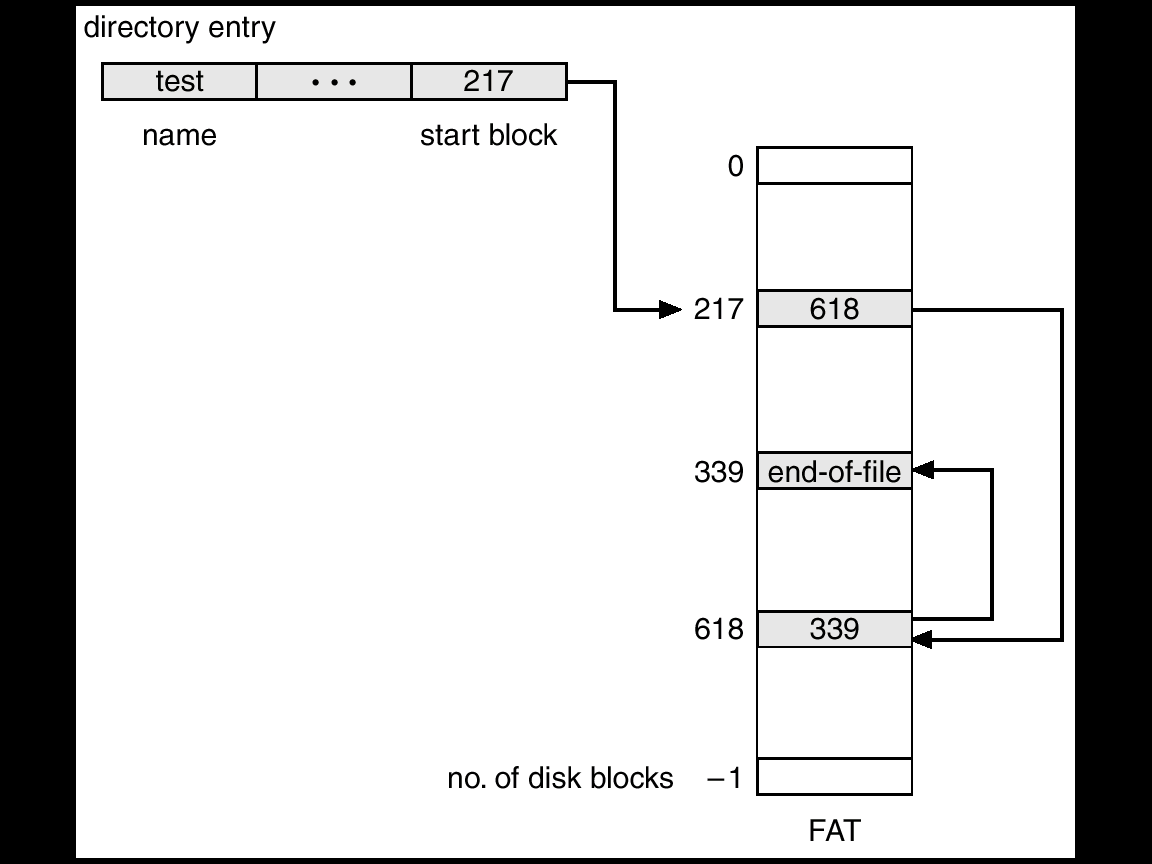
\includegraphics[width=0.55\linewidth]{images/fat_scheme.png} \caption{Schema FAT memoria} \end{figure}

\subsubsection{Overhead di Memoria della FAT}
\qs{Calcolo dello spazio necessario}{
Calcolate lo spazio necessario per memorizzare la FAT di un hard disk con:
\begin{itemize}
    \item Capacità dell’hard disk: 20 gigabyte.
    \item Dimensione di un blocco dell’hard disk: 1 kilobyte.
\end{itemize}
Qual è la percentuale di spazio del disco "sprecata" per memorizzare la FAT?
}

\noindent
Numero di blocchi:
\[
N_{\text{blocchi}} = \frac{20 \times 1024 \times 1024}{1} = 20971520 \, \text{blocchi}.
\]

\noindent
Dimensione della FAT:
\[
\text{FAT} = N_{\text{blocchi}} \times 4 = 20971520 \times 4 = 83886080 \, \text{byte} = 80 \, \text{MB}.
\]

\noindent
Percentuale di spazio occupata:
\[
\text{Percentuale} = \frac{80}{20480} \times 100 \approx 0.39\%.
\]


\nt{
Per risolvere il problema, è necessario determinare il numero di byte richiesti per memorizzare il numero di un blocco dell’hard disk.
}

\subsection{Allocazione indicizzata}

\subsubsection{Descrizione del metodo}
Nell’allocazione indicizzata, si tiene direttamente traccia di tutti i blocchi in cui è contenuto un file memorizzando i loro numeri in un blocco specifico del disco, detto \textbf{blocco indice}.  
\begin{itemize}
    \item Per recuperare i dati di un file, si memorizza tra i suoi attributi il numero del blocco indice.
    \item Questo approccio è simile alla gestione della memoria primaria nei sistemi paginati, in cui il blocco indice funge da \textit{page table}.
\end{itemize}

\subsubsection{Vantaggi}
\begin{itemize}
    \item Come nell’allocazione concatenata, non è necessario che i blocchi siano contigui, evitando così la frammentazione esterna.
    \item L’accesso diretto ai dati del file è particolarmente efficiente:
          \begin{itemize}
              \item Una volta portato in RAM il blocco indice, è semplice calcolare quale blocco dell’elenco contiene il byte desiderato.
          \end{itemize}
\end{itemize}

\subsubsection{Svantaggi}
\begin{itemize}
    \item Per ogni file, è sempre necessario utilizzare un intero blocco indice:
          \begin{itemize}
              \item Se il file è piccolo, gran parte del blocco indice rimane vuota e quindi sprecata.
          \end{itemize}
\end{itemize}

\begin{figure}[h] \centering 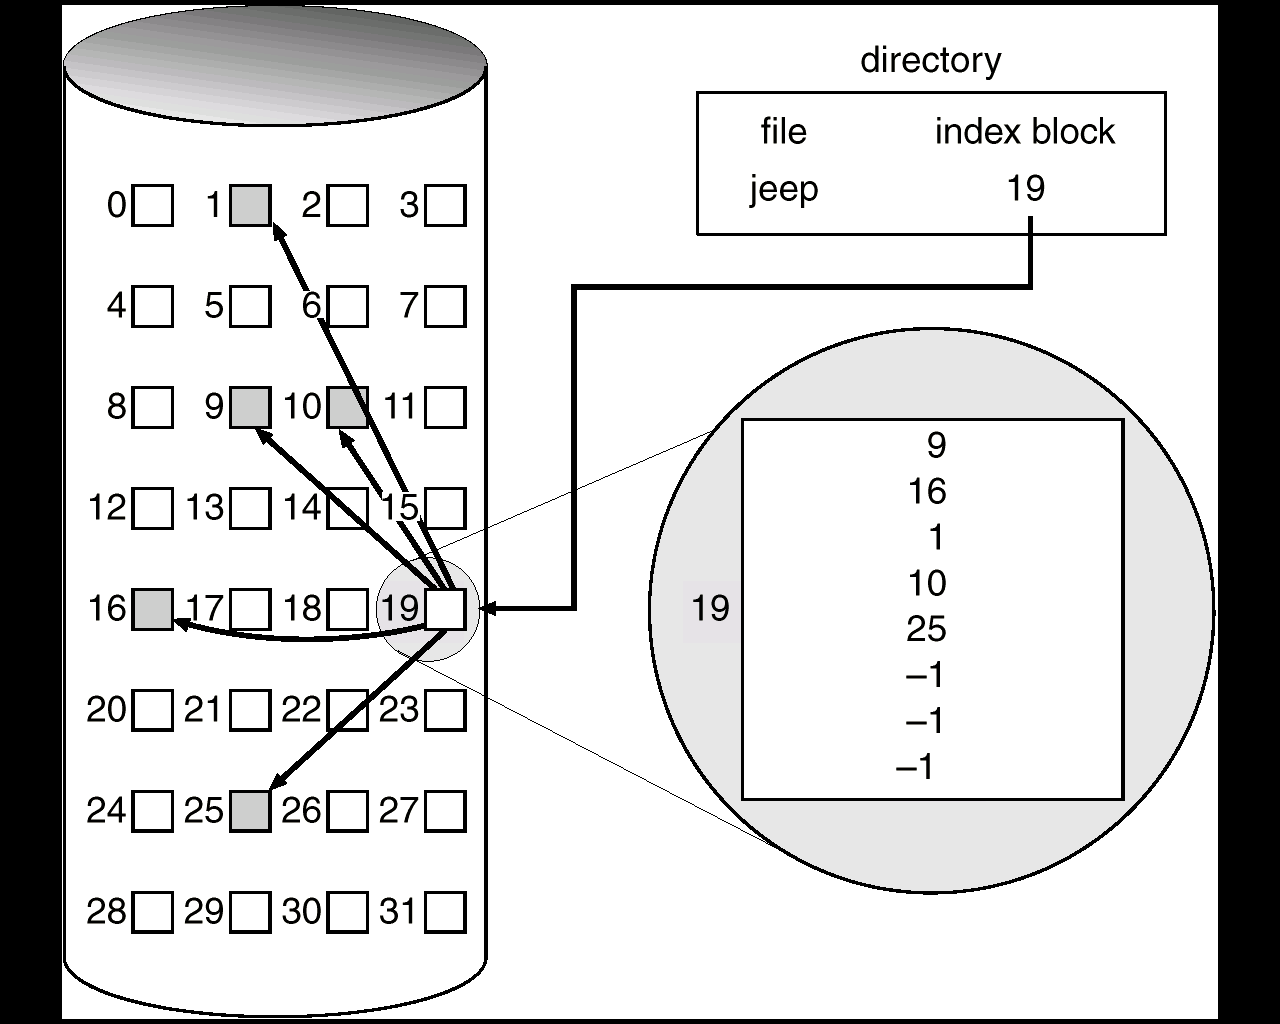
\includegraphics[width=0.50\linewidth]{images/allocazione_indiciz.png} \caption{Allocazione Indicizzata} \label{fig:14.4} \end{figure}

\subsubsection{Problemi e soluzioni}
Un problema rilevante dell’allocazione indicizzata si presenta quando un singolo blocco indice non è sufficiente a memorizzare i numeri di tutti i blocchi dati di un file.  
Le soluzioni principali sono:
\begin{enumerate}
    \item \textbf{Schema concatenato}: l’ultima entry del blocco indice punta a un secondo blocco indice.
    \item \textbf{Schema a più livelli}: il blocco indice contiene esclusivamente puntatori ad altri blocchi indice.
\end{enumerate}

\begin{figure}[h] \centering 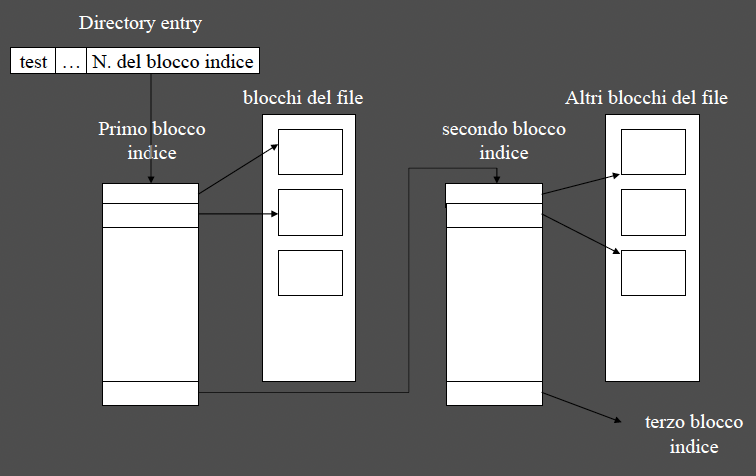
\includegraphics[width=0.50\linewidth]{images/allocazione_indiciz_concatenato.png} \caption{allocazione indiciz concatenato} \label{fig:14.4a} \end{figure}
\begin{figure}[h] \centering 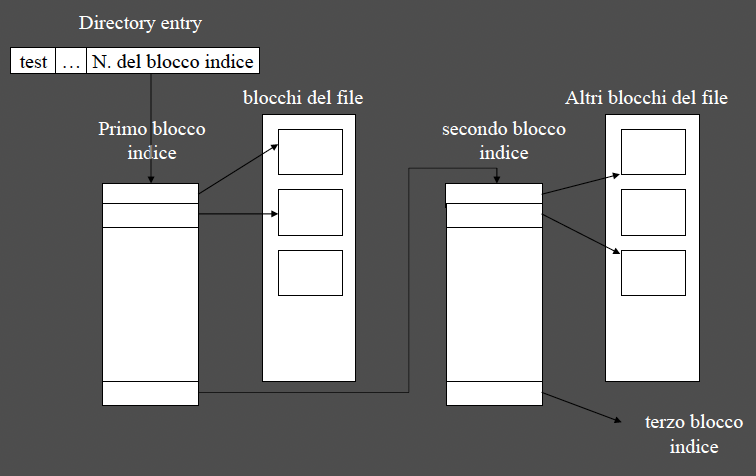
\includegraphics[width=0.50\linewidth]{images/allocazione_indiciz_levels.png} \caption{allocazione indiciz levels} \label{fig:14.4b} \end{figure}
\nt{
    Soluzione esercizio:
    32 bit: 4 byte\\
    1024 blocchi / 4 byte = 256 blocchi\\
    256 blocchi esterni * 256 blocchi interni = 65536 blocchi\\
    65536 blocchi * 1024 byte = 67108864 byte = 64 MB
}
\subsubsection{Gli i-node di Unix}
\nt{
Una variante dell’allocazione indicizzata è utilizzata nei sistemi Unix. In questo caso, ad ogni file è associato un \textbf{i-node} (index-node), che contiene sia gli attributi del file sia l’elenco dei blocchi di dati del file.
}
\begin{itemize}
    \item Gli i-node sono gestiti direttamente dal sistema operativo e vengono memorizzati in modo permanente in una porzione riservata dell’hard disk, solitamente nella prima parte del disco.
    \item Semplificando, i primi blocchi del disco sono dedicati agli i-node di ciascun file.
    \item Quando un file viene registrato in una directory, il numero del suo blocco indice (ovvero dell’i-node) viene associato al nome del file.
\end{itemize}

\subsubsection{Le Directory (richiamo)}
\ref{sec:directory_structure}
\nt{
In Unix, una directory non contiene direttamente gli attributi di un file, ma un puntatore ad una struttura interna, memorizzata in modo permanente sull’hard disk e gestita dal sistema operativo, che include tutte le informazioni relative al file.
}

\ex{Esempio di directory Unix}{
In una directory Unix, ogni file è rappresentato da una struttura come segue:
\begin{itemize}
    \item \texttt{lista.txt} $\rightarrow$ puntatore al relativo i-node (e attributi vari del file)
    \item \texttt{nomi.doc} $\rightarrow$ puntatore al relativo i-node
    \item \texttt{prog.c} $\rightarrow$ puntatore al relativo i-node
    \item \texttt{quake} $\rightarrow$ puntatore al relativo i-node
\end{itemize}
Questa organizzazione consente una gestione efficiente e ordinata dei file.
}

\subsubsection{Organizzazione degli i-node in Unix}
Per tenere traccia di tutti i blocchi di dati di un file, ogni \textbf{i-node} in Unix memorizza diversi puntatori organizzati secondo uno schema gerarchico:
\begin{itemize}
    \item \textbf{10 puntatori diretti}: ciascuno punta direttamente a un blocco di dati del file.
    \item \textbf{1 puntatore single indirect}: punta a un blocco indice, il quale contiene a sua volta puntatori a blocchi di dati del file.
    \item \textbf{1 puntatore double indirect}: punta a un blocco indice, il quale contiene puntatori ad altri blocchi indice, ognuno dei quali punta a blocchi di dati del file.
    \item \textbf{1 puntatore triple indirect}: punta a un blocco indice, che contiene puntatori ad altri blocchi indice, ciascuno dei quali punta a ulteriori blocchi indice che, infine, contengono i puntatori ai blocchi di dati del file.
\end{itemize}

\qs{}{
Se i blocchi sono da 1024 byte e ogni numero di blocco è rappresentato da 32 bit (4 byte), qual è la dimensione massima che un file può raggiungere con questo schema?
}

\cor{Formula della dimensione massima}{
La dimensione massima del file può essere calcolata con la seguente formula:
\[
\text{MaxSize} = 10 \times 1024 + 256 \times 1024 + 256^2 \times 1024 + 256^3 \times 1024 \quad \text{(in byte)}.
\]
}{}

\begin{figure}[h] \centering 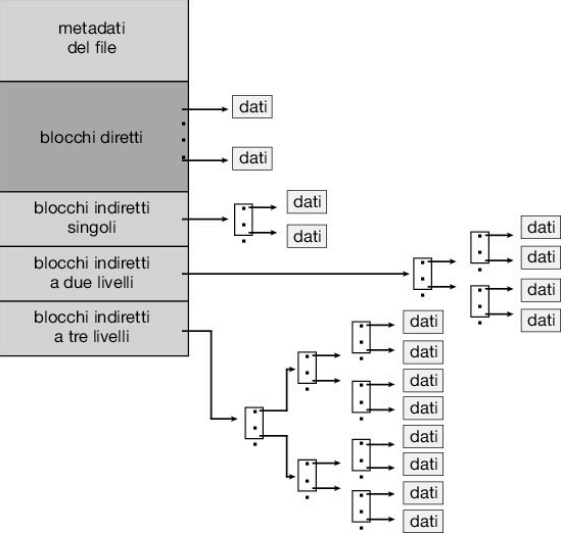
\includegraphics[width=0.50\linewidth]{images/i_node_indicizzati.png} \caption{Allocazione indicizzata: gli i-node} \label{fig:14.8} \end{figure}

\subsection{Il File System NTFS (New Technology File System)}
\subsubsection{Organizzazione e struttura di base}
NTFS, utilizzato dai sistemi Windows (da XP in poi), adotta un approccio simile all'allocazione indicizzata con uno schema concatenato. Le sue principali caratteristiche sono:
\begin{itemize}
    \item Ogni file è descritto da un elemento di dimensione fissa (da 1 a 4 Kbyte, configurabile all’atto della creazione del file system).
    \item Tutti gli elementi del file system sono memorizzati in una struttura chiamata \textbf{master file table (MFT)}, situata nei primi blocchi del disco e gestita esclusivamente dal sistema operativo.
    \item Il numero di un elemento, detto \textbf{file reference}, è associato al nome del file nella directory che lo contiene.
\end{itemize}

\subsubsection{Contenuto di un elemento}
Un elemento NTFS contiene:
\begin{itemize}
    \item Gli \textbf{attributi del file}, tra cui il proprietario, permessi di accesso, dimensioni correnti, date di creazione, accesso, modifica, ecc.
    \item Se il file è molto piccolo, anche i \textbf{dati del file} possono essere contenuti direttamente nell’elemento:
    \begin{itemize}
        \item Questo rende l’accesso al file molto efficiente, poiché è sufficiente leggere l’elemento per ottenere sia gli attributi che i dati.
    \end{itemize}
    \item Se il file è più grande, l’elemento contiene:
    \begin{itemize}
        \item Più puntatori a \textbf{cluster} del disco contenenti i dati del file.
        \item Eventualmente, un puntatore ad un ulteriore blocco di puntatori (schema indicizzato concatenato).
    \end{itemize}
\end{itemize}

\subsubsection{Efficienza e caching}
L’efficienza nell’uso del file system dipende anche dal sistema operativo, che implementa un sistema di \textbf{caching} in memoria primaria dei file e dei loro attributi più usati. Questo approccio prevede che:
\begin{itemize}
    \item Tutte le operazioni sui file e l’aggiornamento degli attributi vengano effettuati accedendo alla copia in RAM dei dati e degli attributi del file.
    \item Il sistema operativo si occupi di mantenere la consistenza tra i dati in RAM e quelli in memoria secondaria, salvando periodicamente le informazioni dal cache sul disco.
\end{itemize}

\section{Hard Link e Symbolic Link in Unix}

\subsection{Hard Link (Link Fisici)}
In Unix, un file è identificato univocamente dall'\textbf{i-node}, che contiene tutte le informazioni relative al file:
\begin{itemize}
    \item Attributi del file (proprietario, permessi, date, ecc.).
    \item Puntatori ai blocchi di dati del file.
\end{itemize}
Il numero dell'i-node (simile a un PID per i processi) identifica univocamente il file all'interno del file system. Tuttavia, per comodità, i file vengono identificati dagli utenti attraverso \textbf{nomi} all'interno delle directory. Ogni nome di file associato a un numero di i-node è definito \textbf{hard link}.

\begin{figure}[h] \centering 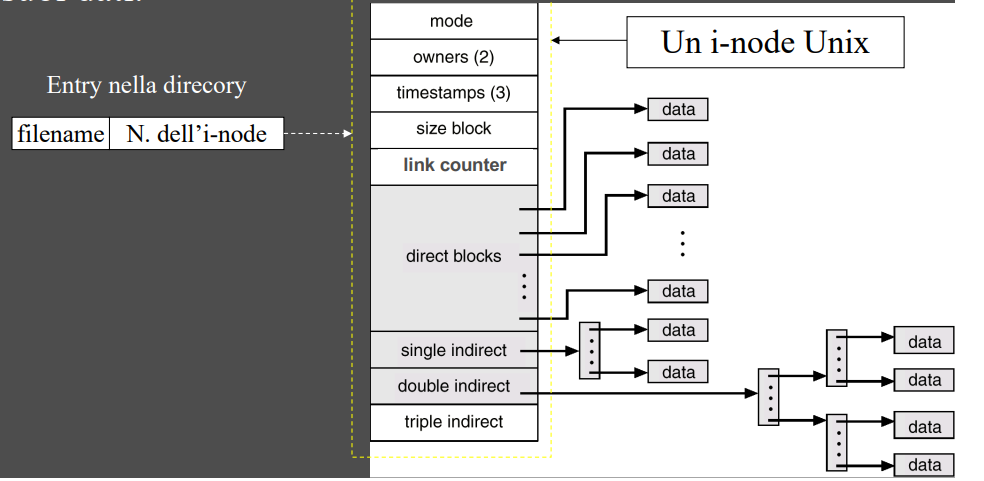
\includegraphics[width=0.50\linewidth]{images/i_node_liinkfile.png} \caption{I-Node} \label{fig:14.4b} \end{figure}

\subsubsection{Caratteristiche principali degli hard link}
\begin{itemize}
    \item Ogni file regolare (non una directory) può avere più hard link, ossia può essere referenziato da più nomi in directory diverse o nella stessa directory (a condizione che i nomi siano diversi).
    \item Gli hard link a un file sono indistinguibili fra loro.
    \item Il numero degli hard link associati a un i-node è tenuto traccia da un campo interno detto \textbf{link counter}.
    \item Se il link counter di un file scende a 0, l'i-node e i blocchi di dati associati vengono rimossi.
\end{itemize}

\subsubsection{Comandi per gestire gli hard link}
\paragraph{Creazione di un hard link}
Si può creare un hard link con il comando \texttt{ln} o con la system call \texttt{link}:
\begin{itemize}
    \item \texttt{ln existing\_file new\_file}
    \item \texttt{link(existing\_file, new\_file)}
\end{itemize}
In entrambi i casi, il sistema operativo:
\begin{enumerate}
    \item Recupera l'i-node di \texttt{existing\_file} e verifica i permessi.
    \item Incrementa il link counter dell'i-node.
    \item Aggiunge una nuova entry nella directory specificata per \texttt{new\_file}, associandola all'i-node di \texttt{existing\_file}.
\end{enumerate}

\paragraph{Rimozione di un hard link}
Gli hard link possono essere rimossi con il comando \texttt{rm} o la system call \texttt{unlink}:
\begin{itemize}
    \item \texttt{rm file\_name}
    \item \texttt{unlink(file\_name)}
\end{itemize}
Il sistema operativo:
\begin{enumerate}
    \item Recupera l'i-node del file e verifica i permessi.
    \item Rimuove l'entry \texttt{file\_name} dalla directory.
    \item Decrementa il link counter dell'i-node.
    \item Se il link counter scende a 0, elimina l'i-node e recupera i blocchi di dati associati.
\end{enumerate}

\subsection{Symbolic Link (Link Simbolici)}
I link simbolici (o soft link) sono un altro tipo di riferimento ai file, simili ai collegamenti utilizzati nei sistemi Windows. A differenza degli hard link:
\begin{itemize}
    \item Un symbolic link è un file speciale che contiene il \textbf{pathname} del file o della directory di destinazione.
    \item È possibile creare symbolic link anche a directory e tra file su volumi o partizioni diverse.
    \item I symbolic link sono distinguibili dagli hard link.
    \item Se il file di destinazione viene rimosso, il symbolic link diventa un puntatore "rotto" (dangling link).
\end{itemize}

\subsubsection{Creazione di un symbolic link}
I symbolic link vengono creati con il comando \texttt{ln -s}:
\begin{verbatim}
ln -s existing_file_or_directory symbolic_link_name
\end{verbatim}
Questo comando:
\begin{enumerate}
    \item Alloca un nuovo i-node per il symbolic link.
    \item Memorizza nel campo \textbf{pathname} dell'i-node il percorso del file di destinazione.
\end{enumerate}

\subsubsection{Differenze tra hard link e symbolic link}
\begin{itemize}
    \item Gli hard link sono più efficienti perché non richiedono di accedere a un i-node aggiuntivo.
    \item I symbolic link sono più flessibili, poiché possono puntare a file su volumi diversi e a directory.
    \item L'eliminazione del file di destinazione non influisce sugli hard link, ma rende inutilizzabili i symbolic link.
\end{itemize}

\subsection{Gestione delle Directory in Unix}
Quando si crea una directory (ad esempio \texttt{newdir} all'interno di \texttt{parentdir}):
\begin{itemize}
    \item La directory contiene automaticamente due entry:
    \begin{itemize}
        \item \texttt{.} che punta all'i-node della directory stessa.
        \item \texttt{..} che punta all'i-node della directory padre.
    \end{itemize}
    \item Il link counter della nuova directory viene inizializzato a 2 (\texttt{.} e \texttt{newdir}).
    \item Il link counter della directory padre viene incrementato di 1 (nuova entry \texttt{..}).
\end{itemize}
\qs{}{
    Leggendo l'i-node di una cartella come facciamo a sapere quante sottocartelle contiene?
}{}
\nt{
    Per sapere quante sottocartelle contiene una cartella, dobbiamo leggere il link counter dell'i-node della cartella stessa.
    Ad esempio, se il link counter è 5, la cartella contiene 3 sottocartelle, oltre a \texttt{.} e \texttt{..}.
}

\subsubsection{Restrizioni sugli hard link alle directory}
Unix proibisce la creazione di hard link a directory diverse da \texttt{.} e \texttt{..} (ad esempio con il comando \texttt{ln}), per evitare la creazione di cicli nel file system. 

\paragraph{Esempio di errore}
Se fosse possibile creare hard link tra directory:
\begin{verbatim}
ln /users newdir // Errore
\end{verbatim}
Si potrebbe generare un loop infinito durante una visita ricorsiva del file system.

\subsection{Conclusione}
Gli \textbf{hard link} e i \textbf{symbolic link} offrono due meccanismi diversi per gestire i riferimenti ai file in Unix:
\begin{itemize}
    \item Gli hard link sono più efficienti, ma meno flessibili.
    \item I symbolic link offrono maggiore flessibilità, permettendo riferimenti a directory e file su volumi diversi, ma con un costo leggermente maggiore in termini di accesso.
\end{itemize}
La scelta tra i due dipende dall'uso specifico richiesto nel file system.
